% Chapter Template

\chapter{OpenCL Background and Related Work} % Main chapter title

\label{Chapter2} % Change X to a consecutive number; for referencing this chapter elsewhere, use \ref{ChapterX}

\lhead{Chapter 2. \emph{OpenCL Background and Related Work}} % Change X to a consecutive number; this is for the header on each page - perhaps a shortened title

%----------------------------------------------------------------------------------------
%	SECTION 1
%----------------------------------------------------------------------------------------

\section{OpenCL Background}

Any OpenCL application typically comprises two distinct program entities - i) the {\em host} which is a single threaded sequential program executing on one CPU core that orchestrates the entire process of managing data and issuing directives for parallel execution, and ii) kernel(s) which execute on devices with support for vector processing (CPU,GPU,FPGA,DSP).  For every computational kernel, the single-threaded host program leverages command queues supported by the OpenCL API to issue commands for  performing the following operations - i) copying the data from host to input buffers resident on device memory (Host to Device or H2D transfer), ii) launching multiple instances of the same kernel to process the data copied to the device and iii) copying back the data stored in output buffers in the device after the kernel has finished processing back to the host memory (Device to Host or D2H transfer). 
	\par As an illustrative example, we consider a simple OpenCL application which performs a vector addition followed by an element-wise trigonometric sine operation. The vector addition kernel $vadd$ executes on device $GPU_0$. It takes as input two input buffers ($b0$ and $b1$) performs element-wise addition and produces an output buffer ($b2$). The kernel $vsin$ executes on device $GPU_1$ and takes one buffer ($b3$) and performs an inplace element-wise sine operation. In Fig. \ref{fig:OpenCLArch}, the OpenCL host program sets up command queues for each GPU device. For $GPU_0$, the host first issues two {\em write} commands ({\tt clEnqueueWrite()}) for buffers $b0$ and $b1$ followed by a {\em barrier} directive ({\tt clEnqueueBarrier()}). The {\em barrier} command in general ensures that all commands enqueued previously finish before proceeding to execute commands enqueued after the barrier. In this case, it is ensured that the write commands are finished before processing the next command in the queue. The host next issues one execute command ({\tt clEnqueueNDRangeKernel()})followed by a barrier directive and finally one read command ({\tt clEnqueueReadBuffer()}) followed again by a barrier directive. We note all the functions with the {\tt clEnqueue} prefix asynchronously issues these commands to the OpenCL runtime system i.e. the host does not have to explicitly wait for a particular command to finish. It simply enqueues the commands and is free to execute  something else while those commands are executed on the target device. 
	\begin{figure}[ht]  
		\centering
		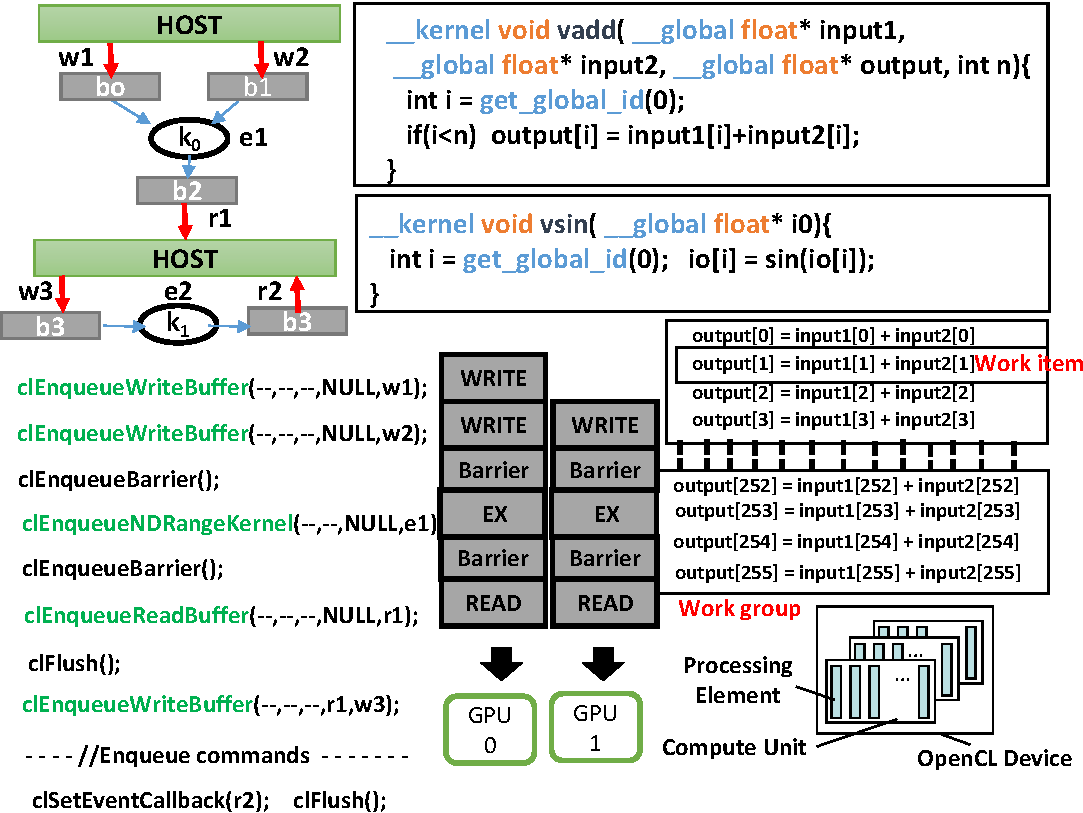
\includegraphics[scale=0.47]{Pictures/OpenCLBackground.pdf}
		\caption{OpenCL Execution \label{fig:OpenCLArch}}
	\end{figure}
	\par The command {\tt clEnqueueNDRangeKernel()} spawns a collection of threads referred as \textit{work items} where each work item executes on a \textit{processing element} on the heterogeneous platform. Each work item is referred by a unique identifier $i$ obtained using the {\tt get\_global\_id()} OpenCL function and is responsible for the addition of  data points in the two input buffers $b0$ and $b1$ ({\tt input1[i]} and {\tt input2[i]} in function call) and storing the result in the corresponding location of the output buffer ({\tt output[i]} in function call). Work items are further grouped into \textit{work groups} and each work group is scheduled for execution on a \textit{compute unit} in an OpenCL compliant device. A \textit{compute unit} may be a Symmetric Multiprocessor(SM) for a GPU device, a single core of a multicore CPU etc. 
	\par Similarly, it may be observed from Fig. \ref{fig:OpenCLArch}, the host issues a write command (for buffer $b3$), the execute command for $vsin$ kernel and one read command (for buffer $b3$ to the command queue pertaining to device $GPU_1$. We note that the write command for $vsin$ can start execution once the read command for the $vadd$ has finished. The OpenCL runtime system  has provisional APIs for specifying dependencies between commands. This is done using {\em events} which are objects that communicate the status of commands issued from the command queue. These events can be used for i) monitoring the execution of read/write operations and kernel execution, ii) enforcing dependencies across multiple commands and iii) notifying the host program about the completion of a command on the device. 
	\par In Fig. \ref{fig:OpenCLArch}, each \textit{write}, \textit{ndrange} and \textit{read} command $c$ enqueued is associated with an event $ev$. This is specified in the last argument of each command $c$ with {\tt clEnqueue} prefix. The second last argument of the function represents events on which the event $ev$ associated with command $c$ is dependent for execution. For our representative example, it may be observed that the event $w3$ is dependent on $r1$. This is specified in the {\tt clEnqueueWriteBuffer} command for buffer $w3$. This is followed by the other enqueue OpenCL function calls such as barriers,   launching the kernel and reading the final output buffer for $vsin$.   
	\par Finally, for the event associated with the last read command in the application (associated with event $r2$ in Fig. \ref{fig:OpenCLArch}), a \textit{callback function} is registered which is responsible for notifying the host when the computation has finished processing on a device. We note the {\tt clEnqueue} OpenCL functions merely enqueue operations to each command queue for the devices. After enqueuing all commands to a command queue, the function {\tt clFlush()} is invoked which informs the OpenCL runtime system to start dispatching the commands pushed to the command queue for execution.  
	\par OpenCL events are thus particularly useful for enforcing read/write and execute dependencies between multiple kernels in application task graphs which are typically represented by a directed acyclic graph (DAG) of OpenCL kernels.  %The state of the art frameworks (StarPU, MultiCL and SOCL) automate the process of setting up command queues and enqueuing commands for computational kernels allowing users to bypass the overhead of implementing boilerplate host code. However, the scheduling heuristics supported by these frameworks are optimized for GPGPU clusters comprising multiple compute nodes with heterogeneous CPU and GPU devices. The mapping decisions offered by these scheduling heuristics typically are coarse-grained in the sense that a single kernel can be mapped to a single device at a time. The supported heuristics do not leverage heuristics for concurrently executing multiple kernels on the same device. This can be achieved by setting up multiple OpenCL command queues on the same device and enqueuing respective write, execute and read commands. 
	We next discuss a slightly more complex DAG example and discuss how  coarse-grained and  fine-grained scheduling decisions result in different command queue configurations in the following subsection. 


\section{Related Work}
\par Given the rich API support by both heterogeneous programming models CUDA and OpenCL, several frameworks have emerged over the last few years with the objective of providing user friendly solutions for development of data parallel applications. Frameworks such as OpenACC \cite{openacc} supports a directive based programming model where relevant annotations in sequential C programs generate data parallel CUDA code for execution on the GPU. Similarly, the framework  HiCUDA \cite{hicuda} is another high level directive based programming language for generating CUDA binaries from sequential C source code. Frameworks such as GMAC \cite{gelado} offer a data centric programming model relieving the end designer from making explicit memory requests while implementing applications. We note that the frameworks discussed are built using the CUDA API and are restricted for use on heterogeneous systems with NVIDIA GPU architectures only. In constrast several OpenCL based frameworks have also been envisioned in the past decade for general purpose heterogeneous programming. 
	\par The most notable framework offering high-level abstractions for developing OpenCL applications is SkelCL \cite{skelCL} which offers algorithmic skeletons for developing data-parallel programs for execution across multiple GPUs. In this context, skeletons refer to higher order functions such as map, reduce, scan etc. which can be leveraged for implementing data parallel algorithms. Note, the primary approach of this work is complementary in the sense that they focus on rapid kernel development , while our work focuses on scheduling optimizations on target heterogeneous architectures. The VirtCL framework \cite{virtcl} provides an abstraction layer between the programmer and the OpenCL runtime system acting as a hypervisor for scheduling multiple OpenCL applications. The abstraction framework leverages a profile driven history based scheduling scheme for dispatching OpenCL kernels on multiple devices.   However a major limitation for VirtCL is that it cannot operate with devices belonging to different platforms. Our framework in contrast is suited to work with different OpenCL platforms and opts for a static based scheduling approach for mapping OpenCL kernels. There also exists frameworks such as SnUCL \cite{snucl}, VOCL \cite{vocl}, MultiCL \cite{multicl} etc. that extend upon the OpenCL runtime API that allow OpenCL applications to leverage devices belonging to heterogeneous clusters.  This work also presents a unified OpenCL implementation by incorporating a task queuing extension layer. However, such APIs still require explicit kernel and host program development and lack support for intelligent scheduling techniques mentioned earlier. 
	\par There also exist unified scheduling frameworks for heterogeneous platforms such as StarPU \cite{augonnet2011starpu} which provides users an interface for designing and experimenting scheduling policies for both CUDA and OpenCL applications. The StarPU runtime system allows users to design scheduling priority functions for experimentation. An extension on StarPU \cite{hugo2014composing} supports scheduling multiple tasks in parallel on a heterogeneous system.  The work reported in \cite{henry2014toward} presents an unified OpenCL implementation called SOCL which directly extends upon StarPU for handling and managing execution of OpenCL workloads across multiple devices using different scheduling policies. The SOCL API typically supports scheduling algorithms that require profiling information for each task on each device in the system beforehand. The most recent work in this domain is reported in \cite{pekka}, which proposes a set of APIs on top of OpenCL using which dependencies can be specified for application DAGs.
	\par Despite the vast number of frameworks available, our proposed framework relies on specification files using which programmers can bypass the overhead of implementing complex host programs and design data parallel applications with ease. We also present a novel software architecture that is capable of automatically extracting both application level and platform level concurrency. Currently the scheduling schemes lack support for performance models necessary for obtaining near-optimal schedules. Future work entails investigating machine learning assisted techniques \cite{grewe2011static,grewe2013opencl,kofler2013automatic,smart,schedcl} for the same. We believe the robust API support in our framework  would allow researchers to investigate these avenues and accordingly design and validate novel scheduling algorithms for heterogeneous platforms.